\chapter[Batteries: Chemical Change into Current]{Batteries: Chemical\protect\\ Change into Current}

\begin{kaichang}
\textbf{Translator safety note:} Do not heat batteries to revive them, or improvise series/parallel connections between mismatched cells. Heating, short circuits, and incorrect installation can cause leakage or injury. Follow the battery and device manufacturers' instructions; see \href{https://oem.energizer.com/english/dos-donts/}{Energizer's battery precautions}.

The television remote has stopped working again. You take out its two AA batteries, rub and warm them in your palms, and put them back. Hey, it changes channels again! But within a few days, it will fail completely.

Before throwing them away, consider a few questions. Each battery says ``\ud{1.5}{V}.'' Where does this electricity come from? Was it poured in at the factory? When a battery is ``used up,'' what exactly is gone: has its electricity leaked away, or has something else run out? And why does rubbing and warming it briefly bring it back to life?

By this chapter's end, you will see that an ordinary battery operates on the same principles as the processes in every cell when you breathe.
\end{kaichang}

\section{Before Looking Inside, See What It Does}

Without dismantling a battery---alkaline batteries contain corrosive substances, so leave them to a recycling facility---we can list its outward behavior:

\begin{itemize}[itemsep=2pt]
\item It has two distinct terminals, marked ``$+$'' and ``$-$''. Reverse them, and some appliances will not work.
\item Connect a small bulb or motor, and current flows continuously. The bulb can shine for a long time: not a brief static-electricity spark, but sustained, steady output.
\item Eventually the bulb dims, the motor slows, and finally it stops. The battery is ``dead.''
\item A dead battery has hardly become lighter, and its case is unchanged. It has not lost something visible.
\item A fresh dry cell has about \ud{1.5}{V} between its terminals. Connect two end to end in series, and the voltage becomes about \ud{3}{V}. Connect them in parallel, and the voltage stays the same, but they supply power longer.
\end{itemize}

Here is something more entertaining: you need not buy a battery at all. Halve a lemon, insert a galvanized nail and a length of copper wire into the flesh, and connect them by wires to a light-emitting diode, an LED. It actually glows faintly! The lemon did not come from a battery factory, so where does its electricity come from?

Together, these observations point to one conclusion: a battery's output is not a mysterious fluid, but \textbf{an ongoing chemical reaction}. When reactants run out, the battery dies. To test this idea, zoom down to the particles.

\section{Putting Redox to Work in Separate Halves}

Chapter 33 discussed reactions driven by electron transfer. Put zinc into copper sulfate solution, and zinc atoms give electrons directly to copper ions. Zinc dissolves as zinc ions, while copper ions become deposited copper atoms. The blue solution slowly fades, reddish copper coats the zinc, and heat is released. Electrons jump straight from zinc to copper, turning all the energy into heat and leaving no useful work.

Now ask a simple question: can we force the electrons to \textbf{take a detour}? Let zinc release electrons in one room and copper ions accept them in another, joined by a wire. The electrons must pass through the wire to get there, making a bulb filament glow along the way. This device that ``separates oxidation from reduction'' is a \textbf{galvanic cell}.

\begin{figure}[htbp]
\centering
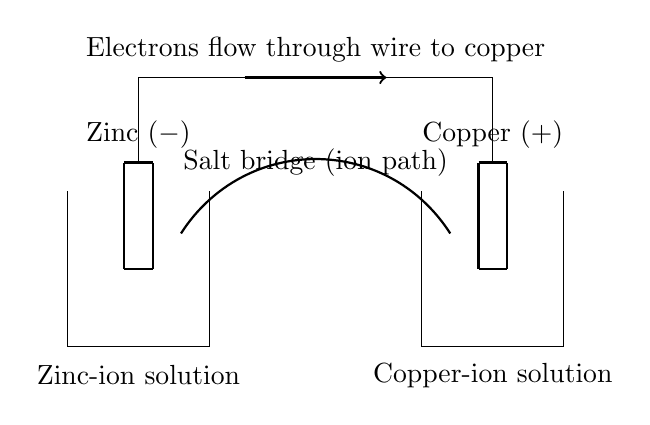
\begin{tikzpicture}[scale=0.9]
% Left beaker
\draw (0,0) -- (0,2.2) (2,0) -- (2,2.2) (0,0) -- (2,0);
\node at (1,-0.4) {Zinc-ion solution};
\draw[thick] (0.8,1.1) -- (1.2,1.1) (0.8,2.6) -- (1.2,2.6) (0.8,1.1) -- (0.8,2.6) (1.2,1.1) -- (1.2,2.6);
\node at (1,3.0) {Zinc ($-$)};
% Right beaker
\draw (5,0) -- (5,2.2) (7,0) -- (7,2.2) (5,0) -- (7,0);
\node at (6,-0.4) {Copper-ion solution};
\draw[thick] (5.8,1.1) -- (6.2,1.1) (5.8,2.6) -- (6.2,2.6) (5.8,1.1) -- (5.8,2.6) (6.2,1.1) -- (6.2,2.6);
\node at (6,3.0) {Copper ($+$)};
% External circuit
\draw (1,2.6) -- (1,3.8) -- (6,3.8) -- (6,2.6);
\draw[->,thick] (2.5,3.8) -- (4.5,3.8);
\node at (3.5,4.2) {Electrons flow through wire to copper};
% Salt bridge
\draw[thick] (1.6,1.6) .. controls (2.5,3.0) and (4.5,3.0) .. (5.4,1.6);
\node at (3.5,2.6) {Salt bridge (ion path)};
\end{tikzpicture}
\caption{A schematic copper--zinc galvanic cell. This is a human-made representation: beaker sizes and salt-bridge shape are not to scale.}
\end{figure}

Three indispensable actions occur simultaneously while it operates:

\begin{itemize}[itemsep=2pt]
\item \textbf{At the zinc electrode}: zinc atoms continually release electrons and enter solution as zinc ions. This is the \textbf{negative electrode}, where electrons start, and its reaction is oxidation.
\item \textbf{At the copper electrode}: electrons arrive along the wire at the copper surface and ``sign off'' approaching dissolved copper ions as copper atoms, plating them onto the electrode. This is the \textbf{positive electrode}, where reduction occurs.
\item \textbf{Inside}: positive charge accumulates on the zinc side and decreases on the copper side. Without balancing, electron flow would soon jam. A salt bridge, a tube filled with an inert salt solution, permits ion migration: anions move toward zinc and cations toward copper, balancing both charge accounts.
\end{itemize}

Notice an easily misunderstood point: \textbf{electrons do not travel through the solution, and ions do not travel through the wire}. Electrons move through metal in the external circuit; ions move through liquid inside the cell. These two ``conveyor belts'' meet at the electrode surfaces, completing a loop. Break any part by disconnecting the wire or removing the salt bridge, and the whole loop stops immediately, freezing the reaction. This is why an old battery with a damaged casing and dried electrolyte is thoroughly dead.

Go one level deeper: why cannot electrons shortcut through the solution? Free electrons move readily only in metals; in water, molecules immediately ``capture'' them, leaving them unable to move. Solutions conduct through whole ions migrating, not electrons racing. A correctly assembled device therefore leaves electrons no choice but the external circuit. Conversely, \textbf{directly} short the terminals with a wire, and electrons flow freely, but the entire energy drop becomes heat in the wire and battery. That explains why short circuits heat up or catch fire, another reminder of Chapter 27's accounting: a free-energy drop must be spent, either as useful work or as heat.

\section{Voltage: An Electron Elevation Difference}

Why do electrons go from zinc to copper, not backward? Chapter 28's free-energy picture still applies: the combination of zinc losing electrons and copper ions gaining them lowers total free energy, so it can happen spontaneously. The metals differ in how readily they surrender electrons, like water surfaces at different heights. Once connected, water flows downhill and electrons flow toward lower energy. This drop is the \textbf{potential difference} read by a voltmeter.

Change the metal pair, and the drop changes: zinc and copper give about \ud{1.1}{V}; magnesium and copper give more, about \ud{2.7}{V}. Connecting cells in series stacks two waterfalls, adding their drops and raising voltage. A battery's printed voltage is therefore not its ``amount of electricity,'' but the reaction's \textbf{size of drop}; how long it lasts depends on its reactant supply.

\begin{qiaoliang}
An alkaline AA cell contains about \ud{3}{g} of metallic zinc. How much charge can it deliver? Zinc's molar mass is approximately \ud{65}{g\cdot mol^{-1}}, so \ud{3}{g} is $3/65\approx 0.046$ mol. Every atom gives up two electrons, yielding about 0.092 mol of electrons. One mole carries about \ud{96500}{C}, the Faraday constant, so total charge is about $0.092\times 96500\approx 8900$ C. Convert to the battery industry's favored unit: $8900/3600$ is about \ud{2.5}{A\cdot h}, exactly the order of magnitude of commercial alkaline AA capacity ratings. You need not memorize battery capacity: count reactants and electrons surrendered per reactant, and the books give the answer.
\end{qiaoliang}

Now symbols can enter. Write the two half-reactions separately:

\begin{itemize}[itemsep=2pt]
\item Negative electrode (oxidation): \[\chem{Zn} \rightarrow \chem{Zn^{2+}} + \chem{2e^-}\]
\item Positive electrode (reduction): \[\chem{Cu^{2+}} + \chem{2e^-} \rightarrow \chem{Cu}\]
\end{itemize}

Add them and cancel electrons on both sides to recover Chapter 33's overall reaction, $\chem{Zn} + \chem{Cu^{2+}} \rightarrow \chem{Zn^{2+}} + \chem{Cu}$. The ledger is unchanged, but electrons now must ``take the outside route,'' converting the free-energy drop into current. A compact cell notation also exists: $\chem{Zn}\,|\,\chem{Zn^{2+}}\,\|\,\chem{Cu^{2+}}\,|\,\chem{Cu}$. Single bars mark phase boundaries, the double bar marks the salt bridge, the negative electrode is left, and the positive electrode right. One line describes the whole device.

\section{A Scientific Dispute Sparked by Frog Legs}

\begin{zhengju}
The battery began with a ``miscarriage of justice.'' In the 1780s, the Italian anatomist Galvani noticed skinned frog legs hanging on brass hooks twitch violently on touching an iron railing, as though revived. Static-electricity experiments were fashionable, and Galvani explained that frogs stored ``animal electricity,'' which metals merely released. His controls showed weaker twitching with one metal and strongest effects with two different metals, reinforcing his belief that electricity belonged to the frog and metals merely conducted it.

His compatriot Volta read the paper but focused on another clue: why two \textbf{different} metals? He suspected the electricity did not belong to the frog at all. Its leg was merely a sensitive ``electroscope,'' with salty tissue conducting current and twitching to reveal it. To refute Galvani, he had to eliminate the frog completely. Volta alternated silver and zinc disks, with saltwater-soaked cloth between pairs, stacking dozens of layers. In 1800, this voltaic pile supplied sustained, steady current without any frog. Humanity had its first continuous electrical source, giving physics a tool for studying steady current. Within the following dozen or so years, water electrolysis and isolation of potassium and sodium depended on it.

Who won? Each was half right. Volta was right that the pile's electricity came from chemical reactions between metals and saltwater, not an animal. But Galvani was not entirely wrong: decades later, nerves and muscles were confirmed to operate with electrical signals, as your heart does now. The mechanism of bioelectricity took much longer to unravel, but it too rests on this chapter's ion migration. Chapter 53 brings an upgraded version. Remember the method: Volta did not stop at ``I disagree,'' but designed an experiment that removed the suspect factor, the frog, leaving only metals and salt as variables.
\end{zhengju}

\section{From Lemons to Lithium: The Battery Family}

Copper--zinc cells are teaching models. Real batteries offer four engineering variations on the same principle:

\begin{itemize}[itemsep=2pt]
\item \textbf{Zinc--manganese dry cells}, ordinary disposable batteries: the zinc casing itself is the negative electrode; a central carbon rod collects current at the positive electrode, whose active material is manganese dioxide. The electrolyte is a paste of ammonium chloride or alkaline solution. Making liquid into paste lets you place the cell sideways or upside down: engineering calls it leak prevention, while the chemistry is unchanged.
\item \textbf{Lead--acid batteries}, used in cars: lead is the negative electrode, lead dioxide the positive, and dilute sulfuric acid the electrolyte. Each cell provides about \ud{2}{V}; six in series make a \ud{12}{V} car battery. Heavy and ungainly, they excel at briefly delivering hundreds of amperes to a starter motor. Cheap, robust, and supported by mature recycling, they remain in use after more than a century.
\item \textbf{Lithium-ion batteries}, in phones and electric vehicles: the negative electrode uses graphite that can host lithium, while positive materials include lithium cobalt oxide or lithium iron phosphate. Their ingenuity lies in moving lithium as \textbf{ions} between two material layers: from negative to positive during discharge, back during charging, while both structural frameworks remain largely intact. This allows thousands of cycles. Lithium is the lightest metal and especially eager to lose electrons, storing several times lead--acid's energy per unit mass: a chemical reason phones can become thinner.
\item \textbf{Fuel cells}: previous batteries seal reactants inside a case, but fuel cells ``feed openly.'' Hydrogen, or hydrogen reformed from natural gas, and oxygen are supplied continuously, surrendering and accepting electrons separately at the catalysts described in Chapter 30. Electrons must take the external circuit, and the sole product is water. More miniature power station than storage tank, a fuel cell keeps producing electricity as long as fuel arrives.
\end{itemize}

Lithium batteries' high energy density comes with a more volatile temperament. Their electrolyte is a flammable organic liquid. An internal short circuit, caused by impact, overcharging, or manufacturing defects, heats rapidly; heat accelerates side reactions, which release more heat. This self-accelerating vicious cycle, ``thermal runaway,'' can ultimately make the whole cell shoot flames. That explains restrictions on power banks in checked aircraft luggage and why swollen phone batteries must immediately be taken out of use. Engineers counter with chemistry and materials: more heat-resistant separators, flame-retardant additives, and less violently heat-releasing positive materials such as lithium iron phosphate. Safety is not merely ``use carefully,'' but a series of molecular-level trade-offs.

A common selection rule emerges: choose not the most ``advanced'' battery, but the one with \textbf{cheap reactants, good reversibility, a large free-energy drop per unit mass, and few side reactions}. More than a century of battery competition has balanced these factors.

There is one more account after a battery ``dies.'' Waste batteries contain metal ions such as lead, cadmium, cobalt, and nickel. Carelessly discarded cells slowly corrode in landfills, letting rain carry ions into soil and groundwater and possibly back into the food chain. Heavy-metal ions tend to accumulate in organisms and disturb enzymes and nerves. Seen differently, however, these pollutants are \textbf{high-grade ore}: a tonne of old lithium batteries contains more cobalt and lithium than a tonne of natural ore. Battery recycling is thus not just an environmental slogan but a real urban-mining industry. Dismantle and dissolve waste batteries, then separate and purify their metals using this chapter's electrolysis and Chapter 35's precipitation and coordination. Now you know why old batteries belong at a recycler: not only to protect land, but to return the raw materials of that energy ``drop'' to industry.

\section{Charging Is Not Just Stuffing Electrons Back}

A rechargeable battery discharges through a spontaneous reaction in one direction. During charging, an external charger applies a larger opposing voltage, \textbf{forcing electrons backward} and reversing the reaction: the positive electrode returns to lead dioxide, or lithium ions return to graphite. Charging consumes electricity from the charger, but no electricity is ``poured into'' the battery or ``used up'' inside it. Chemical substances simply transform back and forth. Chapter 27 established the energy rule: some incoming electrical energy is stored as chemical free energy, while some inevitably dissipates as heat. Not all can be stored, nor all recovered.

Why are not all batteries rechargeable? In disposable alkaline cells, discharge products form difficult-to-reverse new substances: zinc becomes zinc oxide powder, changing shape and location. Forced reverse charging cannot restore the original structure and may generate gas, swelling, or rupture. The charger warning ``never recharge disposable batteries'' has real chemistry behind it.

Even lithium batteries cannot move ions perfectly every time. A tiny fraction gets ``lost,'' reacting with electrolyte or depositing as metallic lithium on the negative surface, gradually reducing usable capacity. Your phone's shorter runtime after two years is not electricity leaking away but fewer lithium ions available to move. Ions move slowly in cold conditions, and large currents produce more side reactions. Reduced winter vehicle range and battery wear from fast charging are all kinetic issues, as in Chapter 29.

\begin{shiyan}
\textbf{Fruit Battery} (safe to make at home).

Materials: a lemon, potato, or apple; a galvanized iron nail with zinc on its surface; thick copper wire or a brass key; several alligator-clip leads; a low-voltage LED; optionally, a multimeter.

Procedure: (1) Insert the nail and copper wire side by side into the fruit, about \ud{2}{cm} apart, making sure they \textbf{do not touch inside}. (2) Connect them separately to the multimeter and read the voltage. (3) Try different fruits and metal pairs, such as two iron nails, and record voltage changes. (4) If you have an LED, connect three or four fruit batteries in series and see whether it lights.

What to observe: zinc and copper give about \ud{0.8}{V} to \ud{1.0}{V}; two identical iron nails give nearly zero. You have personally tested the claim that the drop comes from different metals.

Safety: the very low voltage presents no electric-shock hazard, but \textbf{never} connect any homemade battery to a wall outlet. Metal ions have contaminated the fruit: discard it without eating. Wash your hands afterward.
\end{shiyan}

\section{Electricity in Reverse: Electrolysis and Metals}

A galvanic cell uses a spontaneous reaction to drive electrons. Reverse the power connection and force a nonspontaneous reaction, and you have \textbf{electrolysis}. Turning the principle around supports an entire industrial chain:

\begin{itemize}[itemsep=2pt]
\item \textbf{Electroplating}: suspend an iron nail as the negative electrode in a solution containing copper, nickel, or chromium ions and apply direct current. Copper ions are forced onto its surface and reduced to a dense metal coating, resisting rust and improving appearance. Faucets, keys, and eyeglass frames are often plated.
\item \textbf{Electrolytic aluminum refining}: aluminum loses electrons so readily that it occurs naturally only as oxides, beyond charcoal reduction's reach. Industry dissolves alumina in molten cryolite: pure alumina melts above $2000\,^{\circ}\mathrm{C}$, while cryolite lowers the temperature to about $960\,^{\circ}\mathrm{C}$, saving enormous electricity costs. Powerful current then forces aluminum ions to become liquid aluminum. Once an aristocratic metal dearer than silver, aluminum became commonplace can material only after electrolysis matured. Your drink can is a product of electrochemistry's industrial democratization.
\item \textbf{The chlor-alkali industry}: electrolyzing saturated brine produces three valuable products together: caustic soda, \chem{NaOH}; chlorine, \chem{Cl_2}; and hydrogen, \chem{H_2}. This production line stands behind soap, paper, disinfectants, and the plastic material \chem{PVC}.
\end{itemize}

Keep directions straight: in an electrolytic cell, oxidation occurs at the electrode connected to the power supply's positive terminal, the anode, and reduction at the negative-connected electrode, the cathode. This may seem opposite to galvanic cells' ``negative oxidizes, positive reduces,'' but the universal rule is unchanged: oxidation always occurs at the anode, reduction at the cathode. Only electrode signs reverse with the device's role. If you cannot remember, track electron direction and derive the names instead of memorizing.

\section{Where Does This Model Fall Short?}

Our picture---two half-reactions, an external electron route, voltage as a drop---reliably explains why batteries supply power, but includes simplifications:

\begin{itemize}[itemsep=2pt]
\item \textbf{Voltage is not constant}. The nominal \ud{1.5}{V} is only a fresh battery's nearly unloaded reading. Reactant consumption and product accumulation reduce the drop; a power-hungry appliance also makes voltage sag immediately because internal ion migration cannot keep up, producing internal resistance. Warming an old battery exploits this: higher temperature speeds ions (Chapter 29), briefly raising voltage without adding reactants. It is a final flicker, not resurrection.
\item \textbf{Half-reactions are accounting divisions, not successive steps}. Zinc releasing and copper accepting electrons occur simultaneously at precisely matched rates; asking which comes first is meaningless.
\item \textbf{Voltage does not reveal stored charge}. An almost empty lithium battery can have a resting voltage near that of a full one, then collapse under large current. Remaining charge requires integrating discharge curves, as fuel-gauge chips do, not merely glancing at voltage.
\item A concentration difference alone can produce voltage: the same substance at different concentrations creates a potential difference, a concentration cell. The drop is thus more fundamental than having two metals, as the challenge's Nernst equation explains.
\end{itemize}

\begin{wuqu}
``Batteries contain lots of electrons; appliances use them up, and then the battery is empty.'' This is seductively wrong, partly because everyday language says it. Counterexamples are easy. First, current circulates: the number of electrons leaving and returning to a battery is \textbf{exactly equal}; not one is missing. Appliances consume not electrons but the energy released as they fall from high to low electric potential, just as a waterwheel uses the drop rather than the water. Second, a dead battery still has all its electrons, plentiful in zinc ions and oxidation products. What is exhausted is \textbf{reactants capable of spontaneous reaction}, that reserve of free-energy drop. Replace ``a battery stores electricity'' with ``it stores an unspent chemical drop,'' and your judgment of battery news---capacity, fast charging, degradation---immediately improves.
\end{wuqu}

\section{Back to the Remote's Two Batteries}

Now fulfill the opening promise. ``\ud{1.5}{V}'' is not poured-in electricity, but the free-energy drop of zinc reacting with manganese dioxide. ``Used up'' means not missing electrons, but exhausted zinc donors and manganese dioxide acceptors: the drop flattens, equilibrium is reached, and current stops. Rubbing and warming merely accelerate ion migration and improve contact among remaining reactants, briefly revealing the drop again. They cannot change the total accounts and cannot last: nobody escapes conservation of energy's ledger.

The lemon mystery also resolves: lemon acid supplies hydrogen ions (Chapter 32), the zinc-coated nail loses electrons more readily than copper, and fruit flesh is a natural salt bridge. Your fruit battery and Volta's 1800 pile are the same sort of device.

\section{Countless Batteries inside Your Body}

This chapter converted chemical free energy into electric current. Turn to organisms, and life takes the trick to an extreme. Every cell maintains ion concentration differences across its membrane, with more potassium inside and sodium outside, like a perpetually half-charged miniature battery. A nerve impulse is a rapidly traveling wave of this potential difference reversing along the membrane. Glucose you eat ultimately feeds a mitochondrial electron transport chain: electrons descend step by step, using the drop to pump a proton gradient that makes ATP. The principle is unchanged; proteins and ions replace zinc and copper. In Chapter 51's cell membranes and Chapter 53's cellular respiration, we will return with today's toolkit of half-reactions, potential differences, and ion migration. You will see mitochondria as fuel cells far more intricate than the lithium battery in your phone.

\begin{tiaozhan}
You can skip this without losing the main thread. How do we quantify the drop? Chemists measure a \textbf{standard electrode potential}, $E^{\ominus}$, for each half-reaction relative to a hydrogen electrode, in volts. Subtract tabulated values to obtain cell voltage: $E^{\ominus}_{\text{cell}} = E^{\ominus}_{\text{pos}} - E^{\ominus}_{\text{neg}}$. For copper--zinc, $0.34-(-0.76)$ gives \ud{1.10}{V}. A single conversion links potential and free energy: $\Delta G^{\ominus}=-nFE^{\ominus}$, where $n$ counts transferred electrons and $F$ is the Faraday constant. For nonstandard concentrations, apply the \textbf{Nernst equation}: $E = E^{\ominus} - \dfrac{RT}{nF}\ln Q$, where $Q$ is the product-to-reactant activity ratio. It explains three things together: falling voltage during use as product $Q$ increases; concentration cells, where different $Q$ values on the two sides give $E$; and Chapter 31's conversion between equilibrium constant and voltage, since at equilibrium $E=0$ and $Q=K$. Electrochemistry and thermodynamics shake hands in this equation.
\end{tiaozhan}

\section*{Try It Yourself}

\begin{sikaoti}
\item Draw a particle diagram of a copper--zinc galvanic cell, placing zinc ions, copper ions, and sulfate ions in the appropriate beakers. Mark electron direction in the wire and ion migration through the salt bridge. Note that this is a human-made representation, not ions' real appearance.
\item In the fruit experiment, replacing ``zinc nail $+$ copper wire'' with two identical zinc nails gives almost zero voltage. Explain using free-energy drop, then predict what happens with ``magnesium ribbon $+$ copper wire.''
\item A battery powers a circuit for an hour. Are more electrons entering or leaving the appliance? What does it actually use up? Hint: think of water and a waterwheel.
\item When charging a lead--acid battery, whose role in a galvanic cell does the external power source take? Draw an energy-flow diagram labeling three branches: charger electrical energy, chemical free energy, and dissipated heat.
\item Brine electrolysis and a copper--zinc galvanic cell share the language of electron transfer. Write one sentence for each identifying what drives electrons, and explain the fundamental difference between the two driving forces.
\end{sikaoti}
